\documentclass[11pt,a4paper]{article}
\usepackage[utf8]{inputenc}
\usepackage[T1]{fontenc}
\usepackage{lmodern}
\usepackage[english]{babel}
\usepackage[margin=1in]{geometry}
\usepackage{authblk}
\usepackage{amsmath,amssymb,amsfonts}
\usepackage{graphicx}
\usepackage{booktabs}
\usepackage{xcolor}
\usepackage{hyperref}
\usepackage{cite}
\usepackage{microtype}
\usepackage{fancyhdr}
\usepackage{enumitem}
\hypersetup{colorlinks=true,linkcolor=blue!50!black,citecolor=blue!50!black,urlcolor=blue!50!black,pdftitle={Tokenaholics: The New Silent Addiction of the Artificial Intelligence Era},pdfauthor={Murillo Edson de Carvalho Souza}}
\pagestyle{fancy}
\fancyhf{}
\fancyhead[L]{\small Tokenaholics: autonomy and dependence in the AI era}
\fancyhead[R]{\small\thepage}
\setlength{\headheight}{14pt}
\renewcommand{\headrulewidth}{0.4pt}
\setlist{itemsep=3pt,topsep=5pt}
\emergencystretch=2em
\clubpenalty=10000
\widowpenalty=10000
\displaywidowpenalty=10000
\author[1]{\textbf{Murillo Edson de Carvalho Souza}}
\affil[1]{University of Brasília (UnB)\\Department of Computer Science}
\date{}
\begin{document}
\title{\textbf{Tokenaholics: The New Silent Addiction of the Artificial Intelligence Era}\\[0.5em]\large A Sociotechnical Analysis Using Public Data, Machine Learning, and Consumption Scenarios}
\maketitle
\begin{abstract}
The expansion of generative artificial intelligence makes it necessary to distinguish computational consumption, adoption, and problematic dependence. This article proposes \textit{Tokenaholics} as an exploratory concept without diagnostic equivalence and combines an interdisciplinary critical review with secondary analysis of public aggregates from 2025 and 2026. It examines Anthropic usage profiles by country and occupational group, Vercel daily token and spending shares, and GitHub indicators. K-means using five variables selects a two-group partition among 121 countries, with limited separation (silhouette of 0.308). The GitHub--Anthropic comparison matches eight of the ten countries in the GitHub table. Computer and mathematical occupations have published shares of 23.80\% in chat and 28.17\% in the API in May 2026; these measures retain each channel's denominator. Temporal evaluation of Ridge and three baselines does not support stable predictive superiority. Budget scenarios for 2027 combine token quantity and effective price under a constant mix. The findings describe geographic heterogeneity, differences between channels, and distinct distributions of tokens and expenditure. These results characterize the sociotechnical context without operationalizing or validating Tokenaholics, estimating the prevalence of dependence, or identifying causality. The contribution to computer science is to connect a bounded conceptual definition with reproducible analytical procedures and a future agenda for evaluating regulation, verification, and functional impairment.
\end{abstract}
\noindent\textbf{Keywords:} generative artificial intelligence; language models; overreliance; cognitive autonomy; software engineering; problematic AI use.

\section{Introduction}
An answer appears before the problem has been fully formulated. A piece of code works before its logic has been understood. A second query offers the confirmation that the first did not provide. These situations, used here as hypothetical examples, help formulate a question: when does computational assistance expand the capacity to act, and when does it replace the conditions needed to judge one's own work?

This problem is particularly relevant to computer science. Generative tools participate in code production, documentation, testing, and requirements analysis. The review by Fan et al.\ \cite{fan} situates these applications across software engineering activities and highlights challenges of correctness and verification. The relevant change extends beyond model size: it concerns who formulates objectives, how an answer is tested, and who assumes responsibility for the result.

This article proposes \textit{Tokenaholics} as an exploratory term for investigating potentially problematic operational and cognitive dependence in environments mediated by generative AI. The word refers to the tokens processed by models and deliberately evokes the cultural language of excess. The proposal belongs to the author of this manuscript; this does not establish worldwide lexical priority, exclusive usage, or the discovery of a new disease. The intended contribution lies in the bounded definition and the associated research agenda.

The expression ``new silent addiction'' requires care. ``New'' refers to the technical configuration examined, rather than the absence of earlier forms of technological dependence. ``Silent'' indicates the possibility of harms that delivery metrics may obscure, a hypothesis requiring testing. ``Addiction'' serves as a provocation in the title. The analysis uses problematic use, persistent delegation, and overreliance without assuming equivalence among these categories.

The guiding question is: \textit{how can a proposal about problematic delegation to generative AI be delimited and its usage context characterized without conflating computational intensity, adoption, and clinical dependence?} The general objective is to connect a literature-informed conceptual definition with an empirical characterization of aggregate usage practices. Specifically, the study seeks to: (i) distinguish computational mechanisms and concepts of dependence; (ii) describe national profiles, occupational compositions, and ecological associations between indicators; (iii) compare token and spending shares; (iv) evaluate local share forecasts and budget scenarios; and (v) specify the future evidence needed to investigate problematic use.

The study uses secondary empirical analysis of aggregates, without recruiting participants or applying a clinical scale. It brings together two complementary components: the literature grounds the definition and its proposed dimensions; the data describe the usage context and the limits of computational measurement. The empirical units are countries, occupational groups, and platform share series. There are no individual measures of regulation, understanding, or functional impairment; consequently, the aggregate results do not test the occurrence of Tokenaholics.

\section{Method: Critical Review and Secondary Analysis}
\subsection{Design, Scope, and Selection}
The design combines a critical narrative review based on targeted searches with exploratory secondary data analysis. The thematic core comprises twelve scientific works with formal publication or an identified version between 2022 and 2026. The bibliography includes seventeen additional references, comprising two empirical preprints, reports, datasets, and technical documentation, for a total of 29 entries. Publication year is not treated as the measurement year of every indicator. Exhaustive coverage, a systematic review, and meta-analysis are not claimed.

Searches used academic web resources, publishers' pages, and authors' repositories, prioritizing IEEE Xplore records. English search expressions included \textit{large language models software engineering}, \textit{Copilot security}, \textit{AI overreliance}, \textit{critical thinking generative AI}, \textit{problematic artificial intelligence use}, \textit{anthropological AI}, and \textit{artificial intelligence and work}. Crossref was used to cross-check DOI, authorship, title, publication venue, and dates; institutional repositories and arXiv provided accessible versions. Search results served discovery and did not replace examination of the included sources.

Works were included if they contributed directly to at least one theme: computational mechanisms; performance and verification; cognition and problematic use; or anthropological and social context. Full-text availability and clarity about design and limitations were prioritized. Journalistic claims without a recovered primary basis, unverified commercial tables, and works whose content could not be adequately examined were excluded. The scientific core contains nine contributions from computing and human--computer interaction, one psychology review, one anthropological contribution, and one interdisciplinary social science review. Additional references are identified as preprints, institutional reports, documentation, or datasets according to their nature; they are not uniformly presented as peer-reviewed articles.

Four works were published by IEEE: Pearce et al.\ \cite{pearce}, Fan et al.\ \cite{fan}, Bull and Kharrufa \cite{educacao}, and Assalaarachchi et al.\ \cite{gestao}. Asare et al.\ \cite{asare} appeared at ICSE, a joint IEEE/ACM conference, but the proceedings edition is published by ACM. This distinction avoids classifying every computing contribution as an IEEE publication. Zhou et al.\ \cite{zhou} are explicitly cited as a preprint rather than a peer-reviewed IEEE article.

\subsection{Traceability and Level of Evidence}
For each source, the project records a persistent identifier, retrieval address, accessed version, study type, claim used, and limit of inference. Accessible full texts, metadata, and analytical summaries accompany the project. Formal publication dates were distinguished from deposited-version dates. Thus, the accessible version of Pearce et al.\ predates the 2022 IEEE publication; the bibliographic reference identifies the published work. Assalaarachchi et al.\ have a 2025 accepted version and a 2026 journal issue.

The analysis organizes sources by questions without pooling samples from heterogeneous studies. System results are not treated as effects on people; self-reported associations are not converted into causal cognitive deterioration; and reviews of work do not become clinical evidence. Interpretation distinguishes three levels: findings reported by sources, conceptual connections developed in this article, and proposals that remain untested.

The audit record also flags discrepancies. For Munk et al.\ \cite{munk}, the editorial record and article text list Asger Gehrt Olesen, whereas the institutional repository cover lists Knudsen. Editorial authorship was adopted. The associated erratum was consulted: it corrects the interchange of the images in Figures 3 and 4, which are not reproduced here. This case illustrates why recovering a DOI does not replace inspection of the version consulted.

\subsection{Datasets, Provenance, and Compatibility}
The Anthropic Economic Index provides Claude aggregates by geography and task \cite{aei2025,aei2026}. The study obtained enriched files for the August 2025 week and monthly aggregates for April and May 2026. The 2026 release appeared in June; these are not observations of June or the full year. Direct API data are published globally and exclude Claude Code. Standard Occupational Classification (SOC) categories describe tasks associated with occupations, rather than industrial sectors or users' employment. The \texttt{pct} variable retains the supplier's published percentage for the category node within the relevant geography; it was not renormalized over the selected occupational groups. Collaboration and autonomy indicators are distinct measures with their own definitions.

Vercel provides daily shares by laboratory, model, and metric under CC BY 4.0 \cite{vercelexport}. The export filtered to text modality contains 61 consecutive dates between September and November 2026. It publishes shares, not absolute volumes or dollar amounts. Daily sums for each metric were checked with a tolerance of 0.05 percentage points for rounding. Missing rows were not indiscriminately treated as zero. Descriptive averages and the comparative laboratory panel use series present on all 61 dates; forecast-target selection, described below, uses only the initial window.

Octoverse 2026 supplies reported indicators and country tables \cite{github2026}. Its annual window covers October 2025 through September 2026; totals include public and private repositories unless otherwise stated. Its methodology recalculates earlier years and differs from older editions. Totals from different editions were therefore not simply concatenated. OpenRouter, Stanford HAI, McKinsey, Alphabet, and Portkey reports were used as documented context without adding their coverage universes together \cite{openrouter2026,stanford2025,stanford2026,mckinsey2026,google2025,google2026,portkey2026}.

Three operations were kept separate: joining compatible country tables, contrasting channels within the same dataset, and triangulating sources without a common key. Anthropic's usage index measures share relative to working-age population, not tokens per inhabitant. Input metadata, licenses, revisions, and hashes are recorded in the repository. No private company logs were accessed.

\subsection{Unsupervised Learning and Cross-Source Comparisons}
The May 2026 geographic subset contains 121 countries with five published variables: share of work use, share of formal coursework use, share of collaboration classified as automation, mean autonomy assigned to AI, and estimated human education required by the task. These measures describe usage purpose, collaboration mode, and estimated educational requirements; their selection is exploratory. They are supplier classifications and estimates, rather than clinical assessments, direct observations of competence, or a dependence scale. The per-capita index was not used to construct the groups.

Variables were standardized by mean and standard deviation, and K-means was applied with 30 initializations and seed 42. Values $k=2,\ldots,6$ were compared using silhouette on the exploratory dataset. Stability was evaluated over 30 alternative seeds and 30 random subsamples of 96 countries, the integer part of 80\% of 121 cases, with ten initializations per stability fit. Subsample models assigned labels to the full dataset, compared using the Adjusted Rand Index (ARI). Scaling was retained from the full dataset: the evaluation measures partition sensitivity under that scale, rather than resampling the entire preprocessing procedure. Each country has equal weight. Selecting $k$ does not provide external validation, and standardization does not eliminate correlations between variables.

Descriptive Spearman correlation was calculated between per-capita usage and GDP per working-age person, recovered from the enriched 2025 file using a 2024 economic reference. April and May 2026 index rankings were also compared. Nominal significance values were not interpreted as inference from a worldwide probability sample. An additional ISO-3 join linked the table of the ten largest GitHub account populations to the May Anthropic index, using a 2024 population denominator. Unmatched countries were documented without imputation.

For the occupational contrast, SOC groups were aligned by external identifier between chat/Cowork and API for May 2026. Each share retained its channel denominator. This operation measures relative composition, rather than employment growth, token quantity, or causal effects of assistance.

\subsection{Temporal Forecasting and Sensitivity Analysis}
The forecast target was chosen among laboratories with data on the first 28 dates: the largest mean token share in that window selected DeepSeek. Selection uses neither values nor availability from later dates. After fixing the target, its series was checked for completeness over all 61 dates; a later gap would stop the analysis without silently switching laboratories. Ridge with fixed regularization $\alpha=10$ was compared against persistence, seven-day repetition, and a linear drift based on the mean increment. Ridge uses one-day and seven-day lags, the previous seven-day mean, and a trend; scaling is fitted only on training data. Multistep predictions are recursive and clipped to 0--100\%.

Three forecast origins were used, after 28, 35, and 42 observations, with a 14-day horizon. MAE aggregates 42 errors per method, although the overlapping windows contain only 28 distinct target dates. The 42 errors are therefore not independent observations. The initial Ridge fit has 21 usable rows after lagging. Observations 57--61 were excluded from method selection and form the final five-day test, fitted on the first 56 points. Following evaluation, the method selected by backtesting was updated using all 61 observations to produce a 14-day exercise beyond the sample. Its band uses the 90th percentile of absolute backtest errors; it is descriptive and not probabilistically calibrated.

For 2027, rather than extrapolating 61 days to a full year, budget sensitivity was constructed as $C_1/C_0=(T_1/T_0)(p_1/p_0)$ under a constant mix. Volume multipliers of 1.25 and 1.50 and an illustrative factor derived from an external projection were combined with unit prices of 0.50, 0.75, and 1.00 relative to baseline. These scenarios are separate from the temporal fit and do not estimate observed global consumption.

\section{Tokens, Inference, and Dependence: Computational Distinctions}
\subsection{Processing Unit and Unit of Analysis}
A token is a representation unit used by a model; it does not universally correspond to a word, an idea, or a fixed amount of human effort. Counts depend on the tokenizer, content, and format. For this study, the decisive point is methodological: the same task can produce different counts across systems, and the same count can arise from very different tasks.

In a text application, input, output, and reused context must be distinguished. In tool-using systems, multiple calls can constitute a single task as perceived by the user. Zhou et al.'s preprint \cite{zhou} organizes inference optimizations at the data, model, and system levels and discusses costs associated with model size, attention, and autoregressive generation. This contribution informs the technical description; it is not evidence of behavioral dependence.

At least four quantities need to be separated: processed volume, financial cost, interaction time, and validated outcome. Caching can reduce cost without reducing the information logically mobilized. A long answer can contain little new information. An agent can generate many background calls without a person interacting compulsively. These counterexamples prevent raw volume from serving as a sufficient measure of lost autonomy.

\subsection{An Accounting Model Without Commercial Prices}
To avoid an obsolete table of provider prices, an abstract accounting description is proposed. Consider calls $j=1,\ldots,m$, undiscounted input tokens $I_j$, input billed at a cache rate $K_j$, and billable output $O_j$. For per-million prices $p_{I,j}$, $p_{K,j}$, and $p_{O,j}$:
\begin{equation}
C_{\mathrm{tokens}}=10^{-6}\sum_{j=1}^{m}\left(p_{I,j}I_j+p_{K,j}K_j+p_{O,j}O_j\right).
\end{equation}
The model is an abstraction proposed in this article, rather than a universal description of commercial policies. It assumes mutually exclusive categories and excludes taxes, storage, and tool fees. Additional categories should be incorporated according to service documentation. It is not assumed that every system exposes internal reasoning or that all providers bill it identically.

Even at constant prices, cost per task can grow with call count and repeated context. An application that resends its entire history at every turn can accumulate input without the user writing new material. However, indiscriminate context summarization can remove important constraints and increase rework. The appropriate decision unit is a completed task whose requirements have been met.

A proposed operational indicator is:
\begin{equation}
E_T=\frac{T_{\mathrm{total}}}{N_{\mathrm{validated\ tasks}}},
\qquad N_{\mathrm{validated\ tasks}}>0.
\end{equation}
$E_T$ represents tokens per validated task within a comparable class of problems. It does not measure mental health or individual competence. If no task has been validated, the indicator remains undefined and the failure should be recorded rather than concealed in an average. Comparisons should control for difficulty, artifact size, model, and acceptance criteria.

\subsection{Why More Generation Can Increase Verification Work}
Huang et al.'s review \cite{huang} distinguishes factuality and faithfulness problems and examines hallucination detection and mitigation. It supports a technical precaution: linguistic plausibility does not guarantee correspondence with evidence or instructions. Retrieval resources can support grounding but do not eliminate every failure mode.

The expression \textit{accumulation of pending verification} is proposed for a situation in which artifact production grows faster than evaluation capacity. It describes a workflow rather than a variable measured in this study. Such accumulation can result from organizational pressure, inadequate architecture, or unreflective use; its presence does not identify a specific psychological cause.

In software engineering, this problem arises when the responsible person cannot explain, reproduce, or test a large change. Generated line count ceases to indicate quality. The proposal is to treat requirements understanding, independent testing, and reversibility as components of the outcome. Reducing generation without preserving these components may merely shift costs to future maintenance.

\section{What the Literature Supports and What Remains Open}
\subsection{Code Security: Artifact Risk and Human Performance}
Pearce et al.\ \cite{pearce} investigated 89 scenarios and 1,689 programs generated by an early Copilot version, finding approximately 40\% vulnerable outputs. That rate belongs to the studied dataset and conditions; it does not estimate the insecurity of all AI-assisted code or the prevalence of dependence among programmers. The result demonstrates the need for technical evaluation of generated content.

In a study with 25 participants, Asare et al.\ \cite{asare} observed better security outcomes with Copilot access on the harder problem and no important difference on the easier one. Their unit of analysis is people solving problems with assistance, which differs from isolated automatic generation. The sample and tasks bound generalization. Read together, the studies support rejecting both automatic acceptance of code and the claim that assistance necessarily worsens security.

The conceptual implication is that Tokenaholics needs to be investigated through decision processes and usage consequences. Accepting a correct suggestion after verification can demonstrate competence. Rejecting a useful tool can also worsen the result. The question concerns the capacity to evaluate and regulate delegation under real conditions, rather than the mere presence of AI.

\subsection{Critical Thinking and Overreliance}
Lee et al.\ \cite{lee} analyzed responses from 319 knowledge workers, including 936 usage examples. Greater confidence in AI was associated with less reported exercise of critical thinking; greater task-specific self-confidence was associated with more. They also identified a shift in critical work toward verification, integration, and task stewardship. The self-report design does not demonstrate longitudinal loss of ability. The English-language survey limits direct transfer to the Brazilian context.

Vasconcelos et al.\ \cite{vasconcelos} conducted five studies with 731 participants in total on assisted decisions in maze tasks. Their findings indicate that the effort costs and benefits of verification influence overreliance, and that explanations can help when they facilitate verification. The AI was simulated; the result does not establish a clinical mechanism of chatbot dependence. It offers a design hypothesis: making contestation less costly may be more useful than simply adding explanatory text.

For Tokenaholics, reduced effort requires careful interpretation. It can indicate efficiency, supported learning, or abandonment of evaluation. Distinguishing these possibilities requires observing quality, understanding, and subsequent performance. Asking whether someone ``thought less'' is insufficient, because simplifying a task may be exactly the intended function of the tool.

\subsection{Psychology: Heterogeneity of Problematic Uses}
Dagnino et al.'s scoping review \cite{dagnino} included 37 empirical studies and identified conceptual and measurement heterogeneity. The authors distinguish compulsive or addictive use, cognitive overreliance, and psychological or emotional dependence. Concentration in particular academic contexts and regions limits generalization. The review recommends greater construct clarity and longitudinal and experimental designs; it does not provide a universal rate of AI dependence.

This distinction prevents automatically transferring emotional attachment to an artificial companion to software development practice. Someone can overrely on answers without forming an emotional relationship with the system. Another person can attach emotional value to an interaction while continuing to decide autonomously. A useful concept must accommodate these combinations rather than subsuming them under a single identity of an ``addict.''

For this reason, this article avoids a scored symptom checklist. Anxiety during an outage may reflect a deadline, lost work, or a lack of alternative infrastructure. Investigating impairment requires establishing duration, intensity, realistic possibilities of control, and consequences. Neither frequency, isolated discomfort, nor high cost suffices for clinical classification.

\subsection{Anthropology and Social Sciences of Work}
Munk, Olesen, and Jacomy \cite{munk} discuss a computational anthropology experiment in which classification errors and ambiguities can guide cultural interpretation. The contribution used here is epistemological: understanding a practice requires context, and predictive performance does not equal explanation of meaning. The work does not examine addiction to generative AI. Its connection with Tokenaholics is developed in this article, rather than reported as the authors' finding.

Deranty and Corbin \cite{sociologia} review social science debates on AI and work, including algorithmic management, platform labor, and political and economic conditions. Their argument helps avoid explanations centered solely on individual behavior. The work does not measure token consumption or language-model dependence. The proposed connection is to investigate how productivity expectations and control of work may structure delegation choices.

Consider two professionals with similar consumption. One uses generation to meet team-imposed requirements; the other repeats queries despite already having an adequate solution and recognizing harm. Their telemetry may look equivalent, but the social situations differ. An anthropological investigation would ask how each person defines good work, error, authorship, and legitimate assistance. A sociological investigation would examine targets, hierarchy, resource access, and the distribution of responsibility.

\section{Empirical Results and Evidence Triangulation}
The following subsections distinguish contextualized institutional disclosures from results calculated in this study. Supplier-reported scale and PR indicators are secondary evidence attributed to sources; clustering, correlations, channel contrasts, mean shares, backtests, and scenarios are this study's operations on documented subsets. None of these operations uses a dependence label or outcome.
\subsection{Scale Increases, but Coverage and Periods Matter}
The OpenRouter study analyzes more than 100 trillion tokens and describes task distributions and the adoption of agentic inference; the arXiv publication is dated 2026, whereas the underlying report is from December 2025 \cite{openrouter2026}. This does not automatically confirm weekly figures attributed to September 2026. The report's interaction microdata are not available in the same form as the aggregates used here. No global growth curve was fitted to points lacking a compatible series.

Alphabet reported more than 480 trillion monthly tokens in 2025 and 3.2 quadrillion in its 2026 presentation \cite{google2025,google2026}. Using the rounded benchmarks of 480 and 3,200 trillion yields a nominal ratio of 6.67; comparing 3,200 with the 9.7 trillion cited for two years earlier gives approximately 330. Because of rounding and because the first benchmark was announced as exceeding 480, these ratios illustrate scale rather than exact growth estimates. The numbers cover different products and APIs. Portkey, with different coverage, reports an increase from approximately one billion to one trillion daily tokens in one year \cite{portkey2026}. These disclosures were neither added together nor used as a single time series.

The 2025 AI Index documents a more than 280-fold decrease in inference cost at GPT-3.5-equivalent performance between November 2022 and October 2024 \cite{stanford2025}. This compares inference prices at a performance threshold, rather than a universal price for tasks or models. The 2026 edition extends the economic and adoption context \cite{stanford2026}; its publication date does not turn every indicator into an observation collected in 2026. The relevant argument is that price, capability, adoption, and volume are related but distinct quantities.

In the 2026 McKinsey survey, 80\% of respondents report improved individual productivity, 40\% of respondents from large companies report agents at scale, and approximately 20\% identify constraints from AI operating costs, including tokens \cite{mckinsey2026}. The last percentage does not refer exclusively to tokens. This is a perception and adoption survey, without access to individual consumption or causal validation of productivity. Its percentages were not added as rows in geographic clustering.

\subsection{Countries: Two Exploratory Profiles and the Brazilian Case}
Among the models considered, $k=2$ produced the highest silhouette: 0.308, compared with 0.270 for three groups and 0.285 for four. This indicates limited separation in standardized space, without establishing natural national types. Group 1 contains 69 countries, with means of 42.97\% for work use, 16.42\% for formal coursework, and 47.79\% for collaboration classified as automation. Group 2 contains 52 countries, with 38.02\%, 31.08\%, and 51.88\%, respectively. These are between-country averages, unweighted by conversation volume.

Median ARI across initializations was 0.983. In subsampling, the median was 0.887, but the minimum fell to 0.488: some boundaries are sensitive to composition. The groups describe correlated usage profiles rather than levels of health, competence, or dependence. Classifier-assigned autonomy and automation may carry related information and do not constitute independent measures of a disorder.

\begin{figure}[htbp]
\centering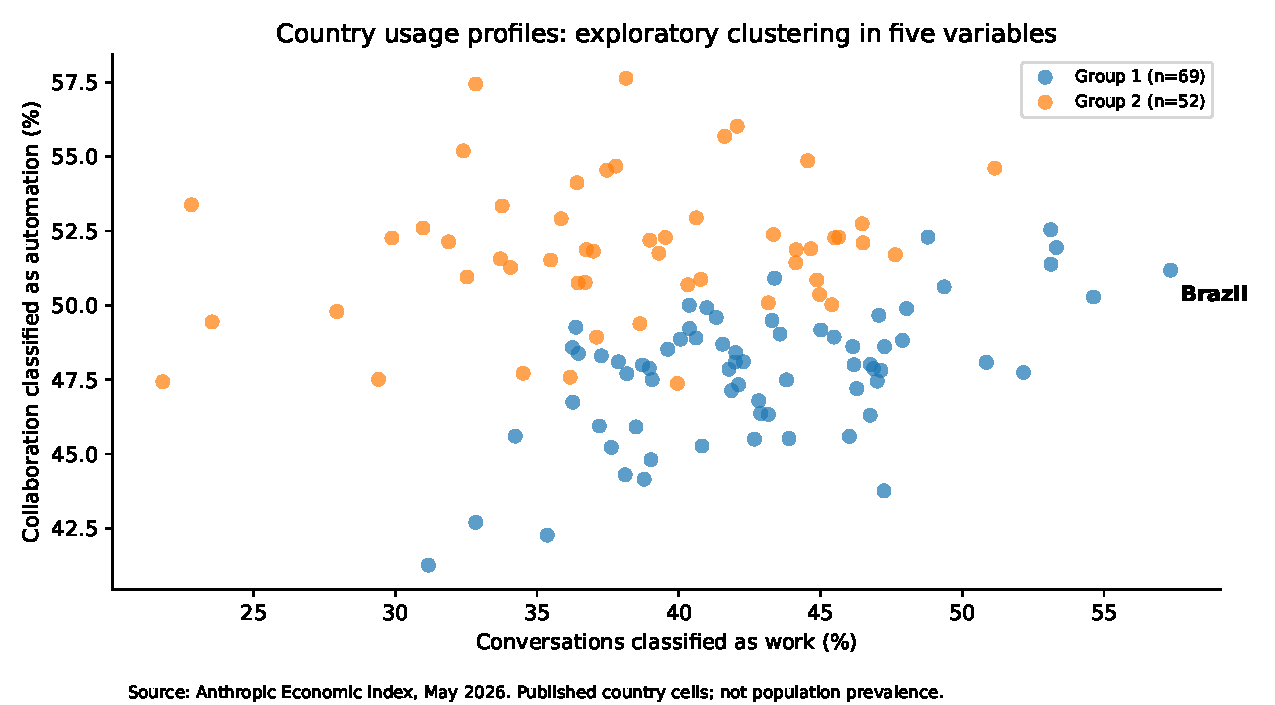
\includegraphics[width=\linewidth]{figures/en/countries.pdf}
\caption{National usage profiles in May 2026. Each point represents a country; colors identify K-means groups calculated from five standardized variables. Axes display two variables on their original scales: work use and collaboration classified as automation, in percent. Source: author's analysis of Anthropic aggregates.}
\label{fig:countries}
\end{figure}

In Figure~\ref{fig:countries}, moving right means a larger share of conversations classified as work; moving upward means a higher proportion of collaboration classified as automation. Every country has an equally sized point, regardless of population or usage volume. Colors identify the 69 countries in group 1 and 52 in group 2. The visualization uses two observed coordinates rather than principal components from principal component analysis (PCA). Because clustering also considers formal coursework, autonomy, and estimated task education, nearby points in this plane can belong to different groups. Overlap is therefore consistent with model construction and limited separation.

Brazil lies to the right of most countries, with 57.35\% work use, and occupies an intermediate position on the automation axis, at 51.18\%. This combination indicates a more professionally oriented profile in the published subset, without identifying the most automated country or demonstrating dependence. The color contrast suggests differences in usage composition; five-dimensional profile comparisons and subsampling stability provide more complete evidence than visual distance between two points.

In Brazil, the share of published usage increases from 2.81\% in April to 3.33\% in May, and the per-capita index rises from 0.86 to 0.96. The latter means usage close to, but still below, the level proportional to working-age population under the index definition. Collaboration classified as automation decreases slightly from 51.51\% to 51.18\%. Brazil belongs to group 1 but cannot be described as more or less ``dependent'' from these indicators. The August 2025 value of 0.926 provides additional context; differences in product, window, and classification prevent inference of a continuous monthly trajectory.

Among 120 countries with compatible economic information, the descriptive Spearman association between GDP per working-age person and the May usage index is 0.931. Among the 114 countries present in April and May, index-rank correlation is 0.996. Persistent rankings and the income association may reflect access, language, prices, and platform selection. Moreover, GDP per person and the usage index involve population normalization, which may contribute to their association and requires caution. These mechanisms and normalization effects were not isolated, and the analysis does not show that income causes problematic delegation.

\subsection{GitHub--Anthropic Comparison: Digital Density and Selection}
The GitHub table of the ten largest account populations has eight matches in the Anthropic geographic subset. China and Russia were unmatched and received no assumed values. Correlation between GitHub accounts per thousand working-age people and the Anthropic usage index is 0.857 in this selected set. Both indicators involve population normalization, numerators and denominators have different dates, and accounts are not unique persons. GitHub account counts are also not restricted to the denominator's age range. The constructed ratio describes relative account density; the correlation is exploratory and ecological across eight cases, rather than a worldwide estimate or individual adoption prevalence.

For Brazil, GitHub reports 10.2 million accounts in September 2026. Combining this figure with working-age population from the baseline file yields approximately 69.44 accounts per thousand people. The coexistence of a strong development presence and an Anthropic index of 0.96 suggests distinguishing digital-community size from relative usage intensity at one supplier. The activities measured on the two platforms cannot be attributed to the same individuals.

\subsection{Occupational Groups: The Channel Changes the Interpretation}
In May 2026, published shares for computer and mathematical occupations are 23.80\% in chat/Cowork and 28.17\% in the API, a ratio of 1.184. In the same group, collaboration classified as automation is 63.90\% and 94.58\%, respectively; this indicator does not have the same meaning as occupational share. Office and administrative support shows 7.89\% and 11.92\%, while education and library occupations show 12.79\% and 6.16\%. The 22 published level-1 SOC groups sum to 98.74\% in chat and 91.56\% in the API. The complementary share was not redistributed, preventing interpretation as a composition renormalized exclusively over those groups.

\begin{figure}[htbp]
\centering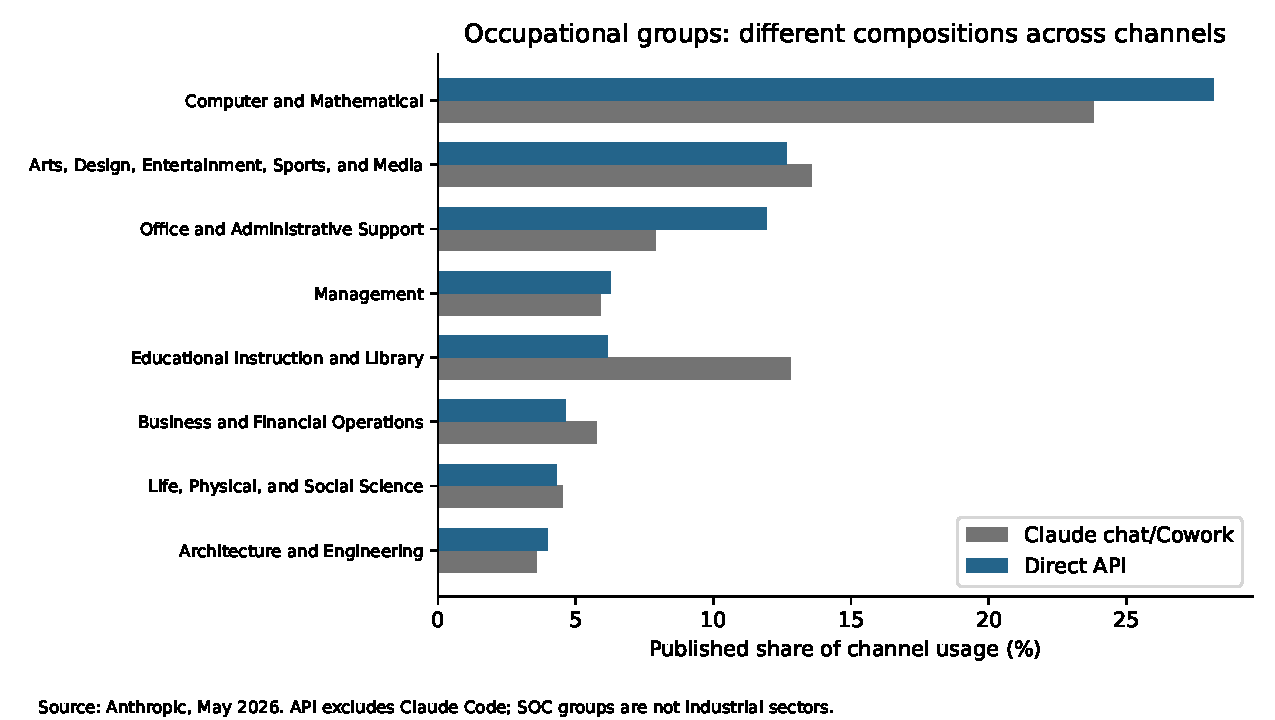
\includegraphics[width=\linewidth]{figures/en/occupations.pdf}
\caption{Occupational composition by channel in May 2026. The eight SOC groups with the largest API shares are shown, ordered by that channel's share. Gray bars represent chat/Cowork and blue bars represent the direct API. Bar lengths indicate the percentage share of the respective channel's classified tasks. Source: author's analysis of Anthropic aggregates. The API excludes Claude Code.}
\label{fig:occupations}
\end{figure}

Figure~\ref{fig:occupations} is read horizontally: the vertical axis identifies occupational groups, while the horizontal axis measures their published share of each channel's usage. Within an occupation, the gap between bars indicates relative channel specialization. Computer and mathematical occupations have the largest displayed share in both channels, with a 4.37-percentage-point advantage in the API; office and administrative support has a 4.03-point API advantage. Education and library occupations, in contrast, have a 6.63-point larger share in chat. The chart thus shows distinct demand profiles consistent with different interfaces and integration methods.

The eight groups were selected by API share, rather than as a complete list of industries or by highest growth. Each bar pair uses two denominators: 28.17\% in the API and 23.80\% in chat do not establish that the API has more computing conversations in absolute terms. Lengths represent occupational share; the automation percentages of 94.58\% and 63.90\% discussed above are a different metric and are not encoded in the bars. Maintaining these distinctions prevents conflating task composition, worker numbers, and delegation intensity.

This contrast helps explain why an enterprise API dashboard can show much greater automation than conversations with people. Changes in composition, tool, and interface offer a competing explanation to presumed growth in dependence. Because the API subset excludes Claude Code, even the computing category does not represent all coding-agent use. Nor should the SOC occupational classification be replaced by the North American Industry Classification System (NAICS) used in Octoverse.

\subsection{Tokens and Spending: Divergent Economic Signals}
Across the 61 Vercel dates, considering only laboratories with complete coverage, DeepSeek's mean daily token share is 37.64\%, but its spending share is 4.95\%. For Anthropic, the figures are 11.58\% and 39.30\%. The ratio of spending share to token share is 0.132 for the former and 3.395 for the latter. This indicator is relative to the gateway mix rather than a list price; daily averages without absolute volumes do not equal cumulative shares over the period.

Vercel's October report, covering September, assigns 71.5\% of tokens and 23\% of spending to open-weight models \cite{verceloctober}. The implied relative averages are $23/71.5=0.322$ for that group and $77/28.5=2.702$ for the remainder: an approximate ratio of 8.40 under the same denominator and period. The mix includes different services and tasks rather than a price experiment with equivalent models. The November report also records decision models at approximately 26\% of requests and 0.53\% of spending \cite{vercelnovember}. Requests, tokens, and expenditure do not produce interchangeable rankings.

As technical support, Bai et al.\ \cite{bai2026}, in a 2026 preprint, analyze trajectories of eight models on agentic coding tasks and identify substantial consumption variability, a strong input contribution, and no simple correspondence between more tokens and greater success. The comparison belongs to the examined benchmarks and configurations rather than every team. The finding reinforces the need to measure resent context, iterations, and final quality instead of assuming long output is the main cost driver.

\subsection{Forecasting: A Baseline Wins, and the Final Test Exposes Instability}
In the 14-day backtest, seven-day seasonal repetition achieves MAE of 5.04 percentage points, followed by Ridge at 5.72, simple drift at 6.47, and persistence at 8.05. The selection based on those windows is retained before observing the final test. On the five reserved days, the seasonal baseline has MAE of 4.72, while persistence reaches 0.88 and Ridge 1.89. Rankings change across different windows and horizons; this does not isolate a cause of the change, but prevents claiming stable predictive superiority for machine learning or any single baseline.

\begin{figure}[htbp]
\centering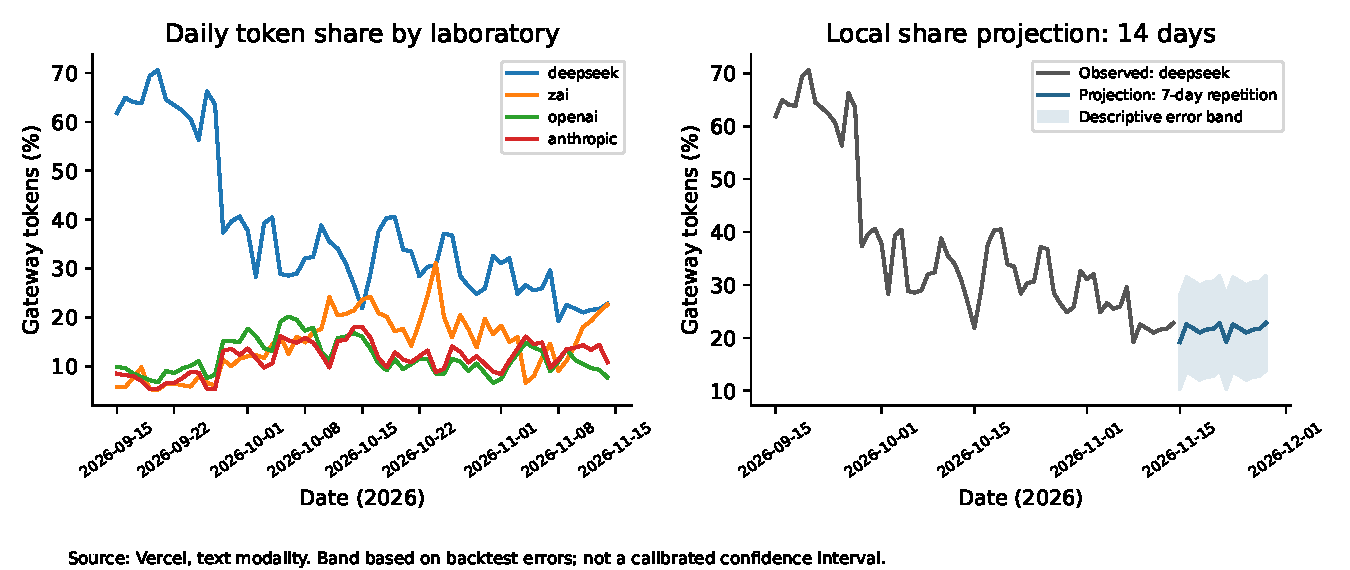
\includegraphics[width=\linewidth]{figures/en/gateway_forecast.pdf}
\caption{Token shares and forecasting exercise for Vercel text modality. Left: daily series of the four laboratories with the highest means and complete coverage. Right: observed DeepSeek series in gray, a 14-day projection using seven-day seasonal repetition in blue, and a descriptive error band. Both vertical scales show percentages of gateway tokens rather than absolute volume. Source: author's analysis of the Vercel snapshot.}
\label{fig:forecast}
\end{figure}

The left panel of Figure~\ref{fig:forecast} describes the relative distribution of tokens across the 61 dates. Each line represents a laboratory and each time point its share of gateway text tokens on that day. DeepSeek's share decreases while other series gain relative ground, but the chart shows only four laboratories: the displayed lines need not sum to 100\%. A declining share can coexist with absolute-volume growth if the gateway total increases. Without daily totals, these curves do not quantify lost demand or global growth.

In the right panel, the gray line reproduces the DeepSeek series used in the experiment; the blue line begins after the final observation and repeats the previous seven days' shares over two weeks. Its periodic shape follows the rule of the baseline selected by backtesting, without demonstrating that a weekly cycle will persist. Shading corresponds to the projection plus and minus approximately 9.02 percentage points, the 90th percentile of absolute backtest errors, bounded at 0 and 100. This band has no validated probabilistic coverage. The change in the best method on the final test recommends treating the figure as short-term sensitivity exploration without extrapolating to 2027 or absolute consumption.

The 14-day extrapolation is presented as a sensitivity exercise rather than a tool ready for investment decisions. The short horizon, five-day final test, and overlapping windows prevent robust uncertainty evaluation. The methodological finding matters: running ML does not require preferring it, and presenting its limitations is part of the scientific result.

\subsection{Resource-Input Scenarios for 2027}
Goldman Sachs publishes a projection of 24-fold growth between 2026 and 2030, reaching 120 quadrillion tokens per month \cite{goldman2026}. This is an external forecast, rather than observed volume or independent validation. Distributing that factor uniformly over four years would yield $24^{1/4}=2.213$ annually. Constant interpolation is an assumption of this article, rather than a specific 2027 forecast attributed to the institution.

Under a constant mix, a 50\% volume increase combined with a 25\% unit-price decrease produces a spending factor of $1.50\times0.75=1.125$, or a 12.5\% increase. If price halves, the same volume produces a 25\% spending reduction. In the illustrative 2.213-factor scenario, even a 50\% price reduction implies approximately 10.7\% budget growth. Lower prices therefore do not guarantee smaller bills when quantity increases.

The scenarios serve budgeting and do not project dependence. Tokens were not directly converted into energy, water, GPUs, or emissions: architecture, modality, caching, utilization, and electricity mix would require additional coefficients absent from the datasets. For team planning, the recommendation is to track quantity per validated task, effective price, latency, rework, and review capacity together rather than rely on a single global multiplier.

\subsection{Pull Requests and Observability: Evidence and Limits}
Octoverse reports 110 million PRs initiated with agent drafts in September 2026, more than 40\% of the total, compared with a 17\% share in March; volume increased approximately sixfold. It also reports 1.3 billion merged PRs and 34.3 billion commits in the annual window \cite{github2026}. PR growth does not measure tokens, useful lines, quality, or loss of control. Initiated PRs and merged PRs have different denominators.

The same report states that, in September, approximately 90\% of agent PRs were merged within two weeks, compared with approximately 86\% of other PRs. This observation does not prove quality, but prevents treating a universal review bottleneck as an inevitable conclusion from the data. The association between agent configuration files and more commits is also not a causal effect: projects and teams may differ in size and prior activity.

Tools such as Langfuse and LiteLLM organize call-level and cost telemetry \cite{langfuse2026,litellm2026}; software availability does not make customer data public. Langfuse's 2026 announcement retiring automatic tokenization estimates further emphasizes that missing usage should remain visible. Incomplete telemetry should not be filled with false precision. Without an auditable public company series, token trends cannot be inferred from commits, PR size, or coauthorship alone.

\section{Tokenaholics as a Sociotechnical Conceptual Proposal}
\subsection{Definition and Boundaries}
The following working definition is proposed:
\begin{quote}
\textit{In this article, Tokenaholics denotes a persistent pattern of delegation to generative AI in which difficulties regulating use are linked to weakened verification, situated autonomy, or recovery capacity, with substantial harm to work, learning, or everyday life.}
\end{quote}
The definition is unvalidated. ``Persistent'' requires temporal investigation; ``substantial harm'' must be documented and contextualized; ``situated autonomy'' means the capacity to formulate and evaluate decisions using legitimately available resources. Autonomy is not assumed to mean doing everything alone. Human collaboration, assistive technologies, and accessibility tools can expand autonomy and should be preserved in evaluation.

It is useful to distinguish infrastructure dependence, functional dependence, and problematic use. The first occurs when a process requires a particular service. The second describes the division of tasks between person and tool, which can be appropriate. The third involves difficulty regulating use and negative consequences. All three can coexist but are not equivalent. A team that stops operating after a service outage may have a continuity problem even when its members retain skills and control over use.

The term should not become a permanent personal label. The preferred unit of analysis is a contextual pattern of practice: a task, a team, a period, and particular access conditions. The same person may use AI judiciously in programming and with little regulation in another activity. This choice reduces stigmatization and supports verifiable interventions.

\subsection{Relationship Between Aggregate Findings and the Proposal}
The findings delimit the context in which a problematic-use hypothesis would need to be investigated. Different national profiles may arise from access, goals, and platform selection; they do not distinguish people who regulate assistance adequately from those experiencing harm. Greater API automation classification characterizes a channel and its tasks without demonstrating weakened user autonomy. The contrast between tokens and expenditure shows that neither volume nor cost is a sufficient substitute for control or well-being.

The absence of stable predictive superiority recommends caution with operational estimates based on short series. This caution is not evidence of compulsion. Testing Tokenaholics would require measures of regulation, verification, understanding, and consequences, followed longitudinally and situated in working conditions. The dimensions below and the future agenda specify this transition from aggregate context to individual or team investigation; they are not variables observed in the models executed here.

\subsection{Proposed Observable Dimensions}
Five dimensions are presented for future research, without weights, thresholds, or diagnostic value:
\begin{enumerate}
\item \textbf{Regulation of use:} ability to stop querying when acceptance criteria are met, respect one's own objectives, and explain why a new call is needed.
\item \textbf{Verification and contestation:} detection of deliberately inserted errors, search for independent evidence, and willingness to reject inappropriate suggestions.
\item \textbf{Understanding and transfer:} ability to explain the solution, adapt principles to a new problem, and distinguish familiar code from code that is merely recognizable.
\item \textbf{Recovery and continuity:} preservation of alternatives proportionate to the activity when a service fails, without requiring manual mastery of the entire computational infrastructure.
\item \textbf{Consequences and context:} effects on deadlines, rework, learning, and well-being, accounting for targets, accessibility, team support, and freedom of choice.
\end{enumerate}
These dimensions deliberately allow divergent outcomes. One participant may have high volume and good regulation; another may have low volume and uncritically accept a high-impact decision. An instrument that classified the former as more dependent solely because of consumption would fail construct validity.

\subsection{A Hypothetical Cycle and Its Alternatives}
The proposed model starts with uncertainty or pressure. A person delegates part of a task, receives an answer, and experiences reduced effort or insecurity. If the answer is incorporated without adequate verification and delivery is rewarded solely for speed, further delegation may become the default response. With fewer opportunities to practice evaluation, perceived difficulty working under alternative conditions may increase. Each transition is a hypothesis; the article does not demonstrate its causal occurrence.

The cycle allows interruptions. An answer can teach a principle and improve later performance. A team can reward failure detection. An interface can make evidence accessible. An experienced professional can deliberately delegate production and concentrate on review. These competing pathways make the proposal testable: if intensive use preserves regulation, understanding, and performance, there is no basis for classifying it as problematic.

``Tolerance'' and ``withdrawal'' are not adopted as established descriptors. Preferring a larger model may arise from a harder task; needing more context may reflect a larger project. Interpreting escalation would require comparing equivalent demands and investigating the purpose of calls. A behavioral hypothesis gains strength only when alternative technical and organizational explanations are considered.

\section{Implications for Systems, Teams, and Computing Education}
\subsection{Architectures Supporting Control and Evidence}
The following recommendations are engineering proposals derived from the conceptual synthesis; they are not treatments, and their effectiveness was not demonstrated in this study. An application can display a per-task budget, call count, and stopping condition. Agents can have iteration limits, explicit scope, and interruption when repeating a failure. The purpose is to make the process observable and controllable.

Generation and acceptance should be separated. An artifact should be considered complete only after checks appropriate to its risk: automated tests, static analysis, dependency inspection, and human review where necessary. Evaluation should have some independence from generation. Asking the same system to confirm its answer does not, by itself, provide this independence. Test cases and external documentation can supply additional criteria without guaranteeing freedom from error.

In the interface, requests for justification can accompany consequential decisions, avoiding friction in every trivial operation. A person can record an initial hypothesis, select what needs checking, and compare alternatives. Making every click difficult can also increase frustration and harm accessibility. Design should evaluate the cost of the control mechanism and its effects on different users.

Context minimization, selective retrieval, and appropriate reuse are efficiency options. Their suitability should be measured by task and quality. Universal token reduction is not recommended as an independent goal: an additional call can prevent a serious failure. Nor is increased generation recommended to demonstrate technological adoption. A budget is an operational limit and an opportunity for reflection rather than a measure of merit.

\subsection{Learning and Preservation of Competence}
Bull and Kharrufa \cite{educacao} propose integrating generative assistants into software development education and discuss scaffolding and fading of support. Their article combines a pedagogical vision with exploratory interviews; it does not demonstrate that a particular program prevents dependence. It helps formulate education in which receiving assistance and learning to evaluate it are simultaneous objectives.

As a proposed extension, an activity could alternate three stages: formulating an initial solution, using AI to explore alternatives, and solving a transfer problem with reduced support. Assessment should observe explanation, testing, and adaptation alongside the final product. Conditions need to accommodate assistive technologies and course objectives. Support should not be withdrawn punitively or without pedagogical justification.

In teams, code reviews can ask which decision was delegated, what evidence supports acceptance, and what remains uncertain. These questions document responsibility and help identify process gaps. Individual inability should not be inferred from a single difficulty explaining something. Observation must consider domain familiarity, available time, and change complexity.

\subsection{Management and Incentives}
Assalaarachchi et al.\ \cite{gestao} analyzed 47 gray-literature sources on generative AI in software project management. The review records opportunities for support and concerns about judgment, privacy, and hallucinations. It describes publicly available practitioner discourse without representing the entire sector or measuring dependence. Its inclusion extends attention to coordination roles beyond code writing.

Productivity indicators should combine time, defects, rework, and maintainability. Counts of prompts, tokens, or generated lines should not replace outcomes. An environment that penalizes questions to colleagues and demands immediate delivery may encourage insufficiently examined delegation; this relationship should be investigated rather than automatically attributed to personal characteristics.

A continuity policy is also relevant: retain decision documentation, executable tests, and service alternatives for critical tasks. The objective is to recover operations and understanding when a tool changes or fails. An organization does not need to reproduce a language model manually to preserve autonomy; it needs to understand its dependence boundaries and the consequences of interruptions.

\section{Future Empirical Agenda: Validation Still Required}
\subsection{Questions and Falsifiable Hypotheses}
The first hypothesis is that regulation and verification explain negative consequences better than raw volume after accounting for difficulty and experience. The second is that an interface with stopping criteria and verifiable evidence reduces acceptance of errors compared with an interface focused solely on generation. The third is that incentives centered exclusively on speed are associated with greater accumulation of pending verification. None of these hypotheses was tested in this manuscript.

An alternative hypothesis is that intensive users develop greater supervisory competence and achieve better transfer outcomes. Another is that recovery difficulties arise mainly from architecture rather than human capacity. A study capable of finding these alternatives is more informative than a questionnaire designed to confirm that all use constitutes dependence.

\subsection{Mixed Design and Longitudinal Evaluation}
The proposal is to follow computing professionals or students over successive periods, with baseline assessment of experience, domain understanding, and tool familiarity. Sample size should be defined through power analysis and feasibility after specifying the effect of interest; no arbitrary number is offered here. Inclusion criteria, outcomes, and the analytical plan should be registered before collection.

An experimental component could compare interfaces and support levels on equivalent tasks, using random allocation and order control where appropriate. Errors inserted to evaluate detection should remain confined to the research environment, with appropriate ethical information and debriefing. The main outcome could be the proportion of detected errors, accompanied by solution quality, time, explanation, and subsequent transfer.

A longitudinal component would investigate within-person change. Repeated measures would help separate task familiarity from possible loss of autonomy. Comparisons under reduced support should preserve essential accessibility resources. Performance without a particular tool should not be treated as a universal measure of intelligence or professional worth.

Interviews and contextual observation would examine why each query occurred, how participants identify sufficient completion, and which organizational demands condition their decisions. This component is necessary to distinguish unproductive repetition from legitimate exploration and interpret the tool's cultural role. Qualitative findings would not automatically become population prevalence estimates.

\subsection{Measurement, Privacy, and Interpretation}
Minimum telemetry could record timestamps, call counts, volume, duration, and validation outcomes per task. Prompt content, proprietary code, and personal data need not be collected by default. Where necessary for the scientific objective, collection would require justification, consent, and appropriate protection. Research should not turn an autonomy proposal into workplace surveillance.

Analyses should account for differences in models, tokenizers, rates, and versions. Comparing counts as equivalent psychological units would be inappropriate. Any future scale would require content assessment, cognitive interviews, structural analysis, consistency assessment, and discriminant validity against work intensity, trust, and experience. No ready-to-use Tokenaholics score is proposed.

If an intervention reduces tokens while worsening quality or accessibility, it should not be considered successful. If it increases queries and improves verification and learning, it may be beneficial. The central criterion is the quality of the relationship between delegation, control, and consequence, with statistical uncertainty made explicit when data are available.

\section{Limitations and Conceptual Responsibility}
Targeted selection of the twelve-work thematic core and seventeen additional references introduces selection bias and does not represent disciplinary consensus. Prioritizing computing and IEEE does not replace specialized searches in clinical or anthropological databases. The empirical datasets involve platform selection, cell suppression, and classified or estimated indicators, without a representative sample of the global market. The GitHub--Anthropic comparison contains eight countries from a table selected by community size. GitHub numerators count user accounts without restriction to the population denominator's ages 15--64, reinforcing that the constructed ratio does not measure population prevalence. Psychological support for the proposal comes mainly from a scoping review and HCI studies rather than original clinical validation.

Repository versions may differ from final publications. Files and metadata were cross-checked, reducing bibliographic risk without assuring complete absence of error; preprints were identified as such. Brazil is examined through secondary analysis without primary collection or a national clinical sample. Methods are exploratory and were not preregistered. Clustering lacks external validation, and stability is conditional on retained scaling; ARI does not quantify classifier errors, rounding, or coverage bias. The short Vercel series, overlapping windows, coverage selection in descriptive comparison, and five-day final test limit predictive evaluation. The displayed band does not incorporate all uncertainty from selection, model changes, or future behavior.

The proposed term may also combine excessively diverse phenomena. If its dimensions do not show coherence or usefulness beyond existing concepts, the proposal should be revised or abandoned. There are risks of stigmatizing assistive use, moralizing productivity, and shifting organizational failures onto individuals. The concept should therefore frame questions about practices and systems rather than classify people.

Finally, ``silent'' does not mean inevitable or invisible to every investigation. It means only that a deliverable can appear satisfactory while part of its verification remains pending. Demonstrating that this configuration is frequent, persistent, and harmful requires dedicated studies. The rhetorical formulation of the title does not replace that demonstration.

\section{Conclusions}
The study connects an exploratory definition of Tokenaholics with characterization of the sociotechnical context of generative AI use. The review grounds distinctions among delegation, overreliance, and dependence; secondary analysis describes country profiles, occupational differences between channels, and distinct distributions of tokens and spending. None of these indicators directly measures regulation of use, understanding, or functional impairment, and the findings do not validate the existence, prevalence, or causes of the proposed pattern.

The contribution to computer science lies in reproducible analysis and examination of measurement limits: clusters show limited separation; occupational shares retain their own denominators; GitHub accounts and Anthropic usage permit only ecological association; and the best forecasting method changes between backtesting and the final test. The 2027 scenarios show conditional quantity and price consequences under a constant mix without estimating future global demand. As a proposal, validated tasks, understanding, and recovery should be evaluated alongside cost; their usefulness in reducing problematic use remains to be tested.

A responsible investigation must allow the proposal to fail: intensive users may retain autonomy and obtain benefits; restrictive interventions may be ineffective or harmful. The scientific commitment is to distinguish these situations through evidence. The challenge posed by Tokenaholics is not to count how much a person talks to a machine, but to understand whether they retain the capacity to direct, evaluate, and interrupt delegation.

\noindent\textbf{Authorship of the conceptual proposal:} Murillo Edson de Carvalho Souza presents the working definition of Tokenaholics in this manuscript. Verified worldwide lexical priority is not claimed.

\medskip
\noindent\textbf{Availability and transparency:} code, redistributable aggregate inputs, results, seeds, metadata, and instructions are provided in the project's \texttt{v0.3.1} research edition: \url{https://github.com/murilloed/tokenaholics-reproducible-study}. This English translation retains that edition's data, results, and scope. Reproduction checks hashes of six inputs, recalculates the analyses, and compares five summaries against a fixed numerical reference using explicit tolerances. Environment and commit are recorded for each run. Access to the private repository requires authorization; the edition has no assigned DOI. Third-party texts remain in the local research archive, with their own links and rights. No participant data were collected. Generative AI assisted research, organization, writing, and translation; the manuscript remains subject to the author's critical review and approval before submission.

\bibliographystyle{IEEEtran}
\bibliography{reference_en}
\end{document}
